%%%%%%%%%%%%%%%
%
% $Autor: Wings $
% $Datum: 2020-01-29 07:55:27Z $
% $Pfad: General/BlueTooth.tex
% $Version: 1785 $
%
%
%%%%%%%%%%%%%%%

\chapter{BlueTooth}

\begin{itemize}
  \item \url{https://www.instructables.com/Arduino-NANO-33-Made-Easy-BLE-Sense-and-IoT/}
  \item \url{https://www.hackster.io/sridhar-rajagopal/control-arduino-nano-ble-with-bluetooth-python-331e33}
  \item \url{https://docs.arduino.cc/tutorials/nano-33-ble-sense/ble-device-to-device}
  \item \url{https://projecthub.arduino.cc/8bitkick/sensor-data-streaming-with-arduino-a6b9f9}
  \item \url{https://www.okdo.com/getting-started/get-started-with-arduino-nano-33-sense/}
  \item \url{https://rootsaid.com/arduino-ble-example/}
\end{itemize}


\begin{figure}
    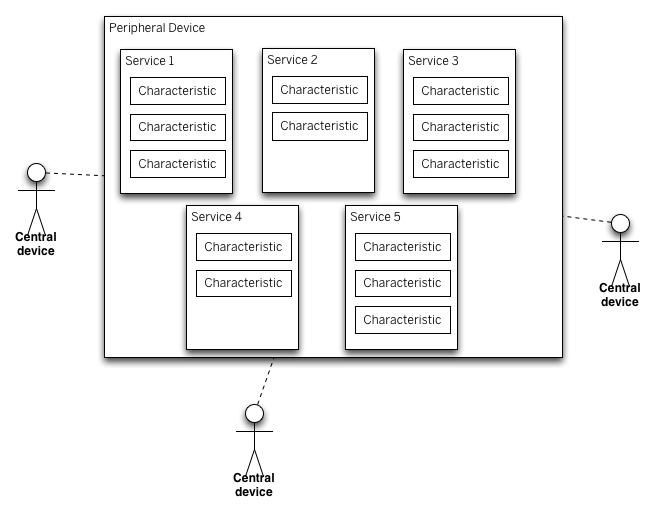
\includegraphics[width=\textwidth]{Bluetooth/BleBulletinBoardModel}
    \caption{BLE Devices -- Peripheral and Central Devices}    
\end{figure}


\section{Quick Start}

This tutorial shows you how to use the free \href{https://www.forward.com.au/pfod/pfodDesigner/index.html}{pfodDesignerV3} V3.0.3774+ Android app to create a general purpose Bluetooth Low Energy (BLE) and WiFi connection for Arduino NANO 33 boards without doing any programming. There are three (3) Arduino NANO 33 boards, the NANO 33 BLE and NANO 33 BLE Sense, which connect by BLE only and the NANO 33 IoT which can connect via BLE or WiFi.
    
Connecting using pfodApp is the most flexible way to connect via BLE (or WiFi). See

Using pfodApp to connect to the NANO 33 BLE (Step 4) and

Using pfodApp to connect to the NANO 33 IoT via BLE (Step 7) and

Using pfodApp to connect to the NANO 33 IoT via WiFi (Step 9) below.
    
owever simple sketches are also provided to send user defined command words via Telnet, for WiFi, or via the free \href{https://play.google.com/store/apps/details?id=com.nordicsemi.nrfUARTv2&hl=en&pli=1}{Nordic nRF UART 2.0} for BLE. See

Using the Nordic nRF UART 2.0 app to connect to NANO 33 BLE (Step 5) and

Using the Nordic nRF UART 2.0 app to connect to the NANO 33 IoT via BLE (Step 8) and

Using a Telnet terminal program to connect to the NANO 33 IoT via WiFi (Step 10) below
    
This tutorial is also available on-line at \href{https://www.forward.com.au/pfod/BLE/Nano33/index.html}{Arduino NANO 33 Made Easy}.


\section{Supplies}

Arduino NANO 33 -- either BLE or Sense or IoT

optionally \href{https://www.forward.com.au/pfod/pfodDesigner/index.html}{pfodDesignerV3} and \href{https://www.forward.com.au/pfod/index.html}{pfodApp}

\section{Step 1: Introduction}

 There are a number of problems with BLE. See this page for \href{https://www.forward.com.au/pfod/BLE/BLEProblems/index.html}{BLE problems and solutions} and there are some \href{https://www.forward.com.au/pfod/BLE/index.html#TroubleShooting}{BLE trouble shooting tips}. The learning curve is steep and the specification has hundreds of specialise connect services each of which requires its own mobile application to connect to. This tutorial shows you how to generate Arduino code for a general purpose Nordic UART BLE connection over which you can send and receive a stream of commands and data to a general purpose BLE UART mobile application. The free \href{https://www.forward.com.au/pfod/pfodDesigner/index.html}{pfodDesignerV3} Android application is used to generate the Arduino code. The output is designed to connect to the paid \href{https://www.forward.com.au/pfod/index.html}{pfodApp} Android application which can display menus, send command, log data and show charts. No Android programming is required. The Arduino code has complete control over what is displayed by pfodApp.
    
For the NANO 33 IoT you can also connect via WiFi. Again the pfodDesignerV3 generates all the Arduino code and by default is designed to connect to pfodApp with optional 128bit security.
    
However you do not need to use pfodApp, you can connect to the generated code using the free Nordic \href{https://play.google.com/store/apps/details?id=com.nordicsemi.nrfUARTv2&hl=en}{nRF UART 2.0} or a Telnet programs (for the WiFi connection). Sketches are included which provide command words to control the boards.
    
The free pfodDesigner V3.0.3774+ will generate Arduino code for a wide range of boards and connection types including Serial connections, Bluetooth Low Energy (BLE), WiFi, SMS, Radio/LoRa, Bluetooth Classic and Ethernet. For examples Arduino code for of a wide range of BLE boards see \href{https://www.forward.com.au/pfod/BLE/index.html}{Bluetooth Low Energy (BLE) made simple} with pfodApp. Here we will be using a BLE connection for NANO 33 BLE, Sense and IoT and a WiFi connection for the IoT.
    
Each of the NANO 33 boards has extra sensor components that differ between the three (3) boards. The pfodDesignerV3 generates code to read/write the digital outputs and perform analogReads and analogWrites. In the examples below we will turn the board LED on and off and read the voltage at A0 and log and plot it. Once that sketch is running you can add each board's specialised sensor libraries and sent their data in place of the analogRead(A0).
    
pfodDesigner generates simple menus and charts, however you can also program custom graphical interfaces in your Arduino sketch. Above is an example of slider control adjusting a guage. All the code for this control is in your Arduino sketch. No Android programming necessary. See \href{https://www.forward.com.au/pfod/pfodControls/index.html}{Custom Arduino Controls} for more examples.
    
\section{How pfodApp is optimised for short BLE style messages}

Bluetooth Low Energy (BLE) or Bluetooth V4 is a completely different version of Bluetooth. BLE has been optimised for very low power consumption. pfodApp is a general purpose Android app whose screens, menus, buttons, sliders and plots are completely defined by the device you connect to.
    
BLE only sends 20 bytes in each message. Fortunately the pfod Specification was designed around very small messages. Almost all of pfod's command are less then 20 bytes. The usual exception is the initial main menu message which specifies what text, menus, buttons, etc. pfodApp should display to the user, but the size of this message is completely controlled by you and you can use sub-menus to reduce the size of the main menu.
    
The \href{https://www.forward.com.au/pfod/pfodSpecification.pdf}{pfod specification} also has a number of features to reduce the message size. While the BLE device must respond to every command the pfodApp sends, the response can be as simple as {} (an empty response). If you need to update the menu the user is viewing in response to a command or due to a re-request, you need only send back the changes in the existing menu, rather then resending the entire menu. These features keep the almost all messages to less than 20 bytes. pfodApp caches menus across re-connections so that the whole menu only needs to be sent once. Thereafter short menu updates can be sent.


\section{Step 2: Creating the Custom Android Menus and Generating the Code}
\begin{figure}
    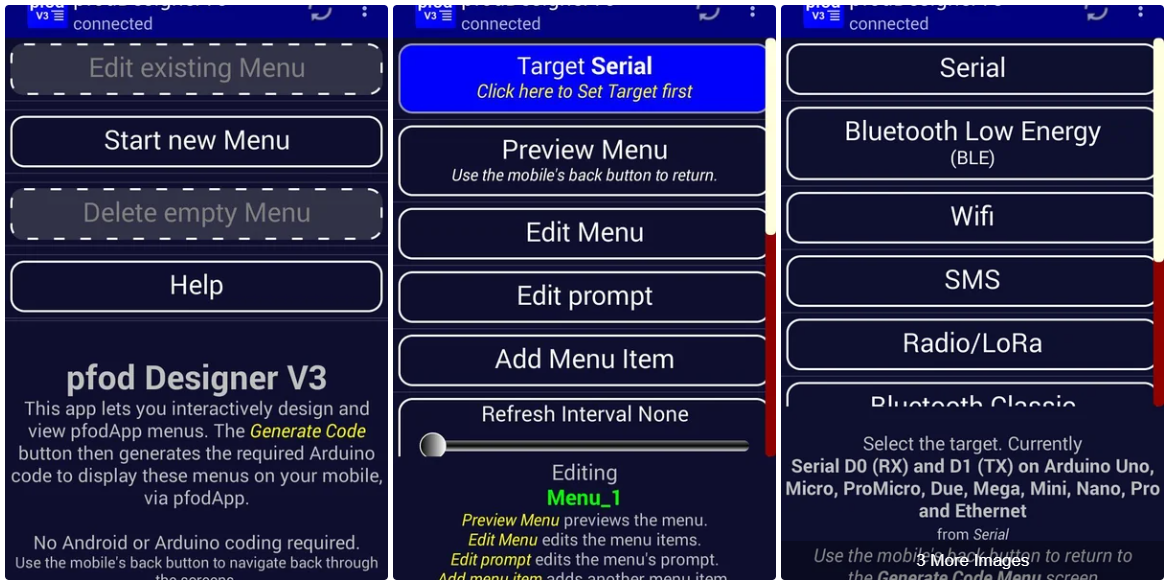
\includegraphics[width=\textwidth]{Bluetooth/AndroidMenu}
    \caption{Step 2: Creating the Custom Android Menus and Generating the Code}    
\end{figure}

Before looking at each of these BLE modules, pfodDesignerV3 will first be used to create a custom menu to turn a Led on and off and plot the voltage read at A0. pfodDesignerV3 can then generate code tailored to the particular hardware you select.

You can skip over this step and come back to it later if you like. The section on each module, below, includes the completed code sketch for this example menu generated for that module and also includes sketches that do not need pfodApp

The free pfodDesignerV3 is used to create the menu and show you an accurate preview of how the menu will look on your mobile. The pfodDesignerV3 allows you to create menus and sub-menus with buttons and sliders optionally connected to I/O pins and generate the sketch code for you (see the pfodDesigner example tutorials) but the pfodDesignerV3 does not cover all the features pfodApp supports. See the pfodSpecification.pdf for a complete list including data logging and plotting, multi- and single- selections screens, sliders, text input, etc.

Create the Custom menu to turn the Arduino LED on and off and Plot A0
Start a new menu and select as a target Bluetooth Low Energy (BLE) and then select NANO 33 BLE (and Sense). pfodDesignerV3.0.3770+ has support for NANO 33 boards.

Then follow the tutorial Design a Custom menu to turn the Arduino Led on and off for step by step instructions for creating a LED on/off menu using pfodDesignerV3.

If you don't like the colours of font sizes or the text, you can easily edit them in pfodDesignerV3 to whatever you want and see a WYSIWYG (What You See Is What You Get) display of the designed menu.

Now we will add a Chart button to display the A0 reading. The steps to does this in pfodDesignerV3 are shown in Adding a Chart and Logging Data The AtoD range is 0 to 1023 for 0 to 3.3V

Generating the code from pfodDesignerV3 gives the this sketch \FILE{Nano33BLE\_Led\_A0.ino}

% Hier weiter: https://www.instructables.com/Arduino-NANO-33-Made-Easy-BLE-Sense-and-IoT/

\section{BLE Mobile App ``Nordic Semiconductors nRF Connect''}

\begin{itemize}
  \item On your mobile, install the App ``Nordic Semiconductors nRF Connect''. There are Android and IOS versions.
  \item In the Arduino IDE open Serial Monitor by clicking on the magnifying glass icon on the top right.
\end{itemize}

The Nano will start sending BLE advertising packets and wait for a Central (Mobile Phone) to connect.

\begin{center}
  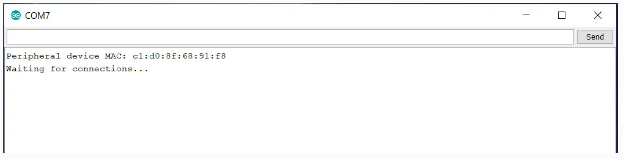
\includegraphics[width=\textwidth]{BlueTooth/BlueToothApp01}
  \captionof{figure}{App nRF  is searching the Arduino Nano BLE Sense}
\end{center}

\medskip



In the App nRF on your mobile select \textbf{Scan} and you should see \textbf{Nano33BLE} as a device you can connect to.

Attention: BLE Peripherals can only connect to one device at a time -- if the Nano33BLE is already connected it could be to another device nearby.

\begin{center}
  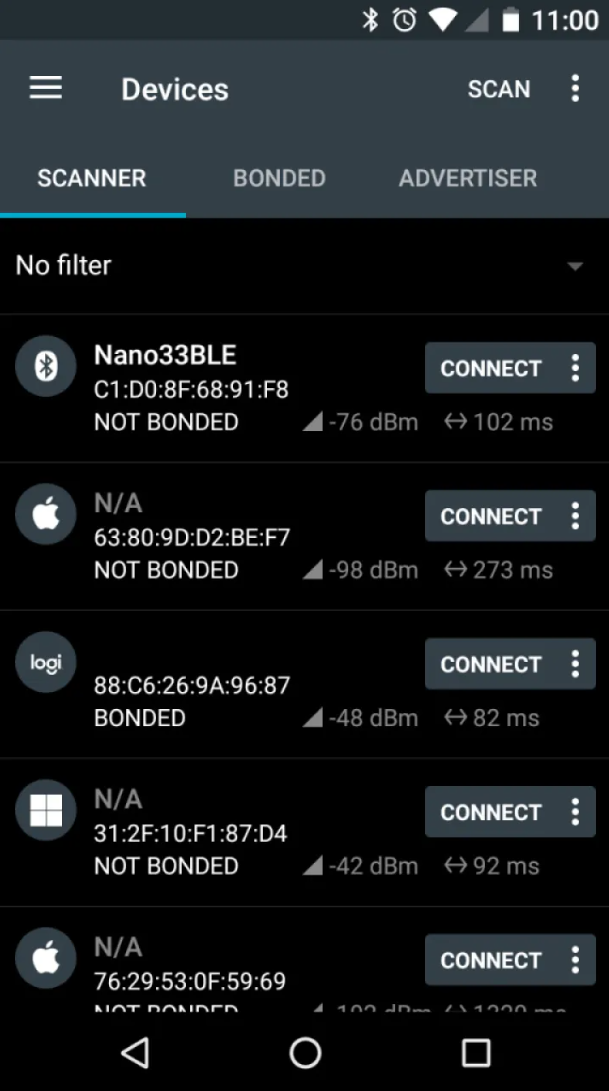
\includegraphics[scale=0.3]{BlueTooth/BlueToothApp02}
  \captionof{figure}{App nRF  is searching the Arduino Nano BLE Sense}
\end{center}

\medskip

Connect to the Nano and select the Unknown Service.

\begin{center}
  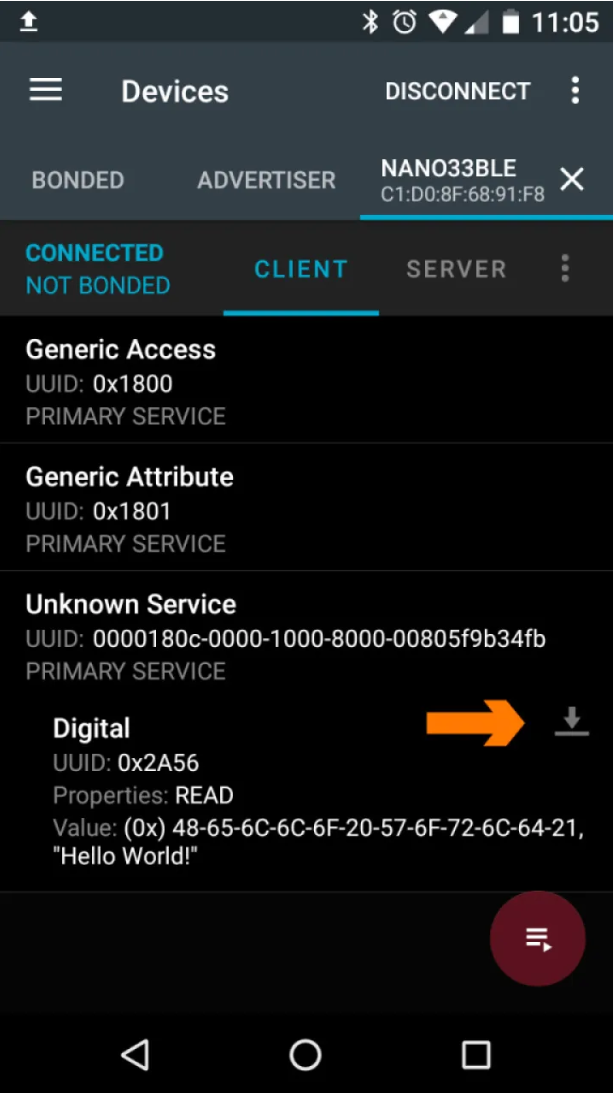
\includegraphics[scale=0.3]{BlueTooth/BlueToothApp03}
  \captionof{figure}{App nRF  is getting data the Arduino Nano BLE Sense}
\end{center}

\medskip

Touch the \textbf{down arrow} next to the characteristic \textbf{Digital}  and it will read the message ``Hello World!'' being broadcast by the Nano33BLE.


\section{Arduino BLE Example -- Explained Step by Step}


\subsection{Arduino BLE Example Code Explained}

In this tutorial series, I will give you a basic idea you need to know about Bluetooth Low Energy and I will show you how you can make Arduino BLE Chipset to send and receive data wirelessly from mobile phones and other Arduino boards. Let's Get Started.


Arduino Nano 33 BLE Sense, Nano with BLE connectivity focussing on IOT, which is packed with a wide variety of sensors such as 9 axis Inertial Measurement Unit, pressure, light, and even gestures sensors and a microphone.

 It is powered by Nina B306 module that supports BLE as well as Bluetooth 5 connection. The inbuilt Bluetooth module consumes very low power and can be easily accessed using Arduino libraries. This makes it easier to program and enable wireless connectivity to any of your projects in no time. You won’t have to use external Bluetooth modules to add Bluetooth capability to your project. Save space and power.
 
\subsection{Arduino BLE – Bluetooth Low Energy Introduction}

BLE is a version of Bluetooth which is optimized for very low power consuming situations with very low data rate. We can even operate these devices using a coin cell for weeks or even months.
 
 Arduino have a wonderful \href{https://www.arduino.cc/reference/en/libraries/arduinoble/}{introduction to BLE} \Mynote{cite} but here in this post, I will give you a brief introduction for you to get started with BLE communication.
 
 Basically, there are two types of devices when we consider a BLE communication block.
 
\begin{itemize}
  \item The Peripheral Device
  \item The Central Device
\end{itemize}

Peripheral Device is like a Notice board, from where we can read data from various notices or pin new notices to the board. It posts data for all devices that needs this information.

\begin{figure}
  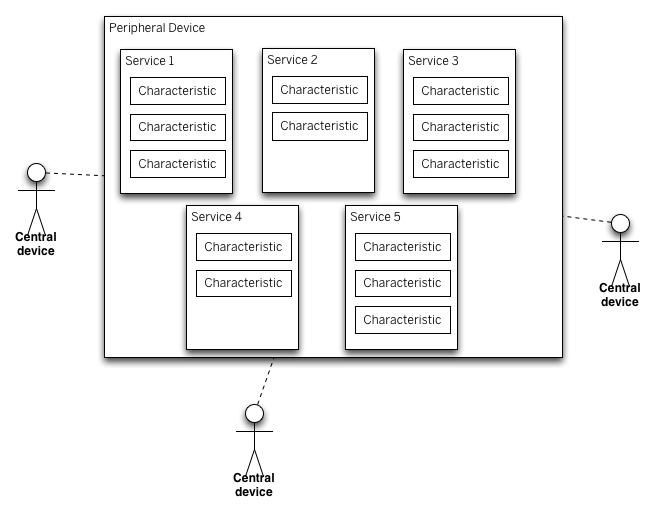
\includegraphics[width=\textwidth]{Bluetooth/BleBulletinBoardModel}
  \caption{BLE Devices -- Peripheral and Central Devices}    
\end{figure}


Central Devices are like people who are reading notices from the notice board. Multiple users can read and get data from the notice board at the same time. Similarly multiple central devices can read data from the peripheral device at the same time. 

The information that is given by the Peripheral devices are structured as Services. And These services are further divided into characteristics. Think of Services as different notices in the notice board and services as different paragraphs in each notice board.

If Accelerometer is a service, then their values X, Y and Z can be three characteristics.

Now let's take a look at a simple Arduino BLE example. 

\subsection{Arduino BLE Example 1 -- Battery Level Indicator}

In this example, I will explain how you can read the level of a battery connected to pin A0 of an Arduino using a smartphone via BLE. This is the code here. This is pretty much the same as that of the example code for Battery Monitor with minor changes. I will explain it for you.

First you have to install the library ArduinoBLE from the library manager.

Just go to \FILE{Sketch -> Include Library -> Manage Library} and Search for \PYTHON{ArduinoBLE} and simply install it.

\subsection{Arduino BLE Tutorial Battery Level Indicator Code}

\begin{code}
\begin{Arduino}
#include <ArduinoBLE.h>
BLEService batteryService("1101");
BLEUnsignedCharCharacteristic batteryLevelChar("2101", BLERead | BLENotify);

void setup() {
    Serial.begin(9600);
    while (!Serial);
    
    pinMode(LED_BUILTIN, OUTPUT);
    if (!BLE.begin()) 
    {
        Serial.println("starting BLE failed!");
        while (1);
    }
    
    BLE.setLocalName("BatteryMonitor");
    BLE.setAdvertisedService(batteryService);
    batteryService.addCharacteristic(batteryLevelChar);
    BLE.addService(batteryService);
    
    BLE.advertise();
    Serial.println("Bluetooth device active, waiting for connections...");
}

void loop() 
{
    BLEDevice central = BLE.central();
    
    if (central) 
    {
        Serial.print("Connected to central: ");
        Serial.println(central.address());
        digitalWrite(LED_BUILTIN, HIGH);
        
        while (central.connected()) {
            
            int battery = analogRead(A0);
            int batteryLevel = map(battery, 0, 1023, 0, 100);
            Serial.print("Battery Level % is now: ");
            Serial.println(batteryLevel);
            batteryLevelChar.writeValue(batteryLevel);
            delay(200);
            
        }
    }
    digitalWrite(LED_BUILTIN, LOW);
    Serial.print("Disconnected from central: ");
    Serial.println(central.address());
}
\end{Arduino}
\caption{Arduino BLE Tutorial Battery Level Indicator Code}

\end{code}


\subsection{Arduino Bluetooth Battery Level Indicator Code Explained}

\begin{lstlisting}
#include <ArduinoBLE.h>
BLEService batteryService("1101");
BLEUnsignedCharCharacteristic batteryLevelChar("2101", BLERead | BLENotify);
\end{lstlisting}

The first line of the code is to include the file \FILE{ArduinoBLE.h}. Then we will declare the Battery Service as well the battery level characteristics here. Here we will be giving two permissions  -- \PYTHON{BLERead} and \PYTHON{BLENotify}. 

\PYTHON{BLERead} will allow central devices (Mobile Phone) to read data from the Peripheral device (Arduino).  And BLENotify allows remote clients to get notifications if this characteristic changes. 

Now we will jump on to the Setup function.

\begin{lstlisting}
Serial.begin(9600);
while (!Serial);
pinMode(LED_BUILTIN, OUTPUT);
if (!BLE.begin()) {
    Serial.println("starting BLE failed!");
    while (1);
}
\end{lstlisting}

Here it will initialize the Serial Communication and BLE and wait for serial monitor to open. 

Set a local name for the BLE device. This name will appear in advertising packets and can be used by remote devices to identify this BLE device.

\begin{lstlisting}
BLE.setLocalName("BatteryMonitor");
BLE.setAdvertisedService(batteryService);
batteryService.addCharacteristic(batteryLevelChar);
BLE.addService(batteryService);
\end{lstlisting}

Here we will add and set the value for the Service UUID and the Characteristic.

\begin{lstlisting}
BLE.advertise();
Serial.println("Bluetooth device active, waiting for connections...");
\end{lstlisting}

And here, we will Start advertising BLE.  It will start continuously transmitting BLE advertising packets and will be visible to remote BLE central devices until it receives a new connection.

\begin{lstlisting}
BLEDevice central = BLE.central();
if (central) {
    Serial.print("Connected to central: ");
    Serial.println(central.address());
    digitalWrite(LED_BUILTIN, HIGH);
\end{lstlisting}

And here, the loop function. Once everything is setup and have started advertising, the device will wait for any central device. Once it is connected, it will display the MAC address of the device and it will turn on the builtin LED.
    
\begin{lstlisting}
    while (central.connected()) {
        int battery = analogRead(A0);
        int batteryLevel = map(battery, 0, 1023, 0, 100);
        Serial.print("Battery Level % is now: ");
        Serial.println(batteryLevel);
        batteryLevelChar.writeValue(batteryLevel);
        delay(200);
    }
\end{lstlisting}

Now, it will start to read analog voltage from A0, which will be a value in between 0 and 1023 and will map it with in the 0 to 100 range. It will print out the battery level in the serial monitor and the value will be written for the batteryLevelchar charecteristics and waits for 200 ms. After that the whole loop will be executed again as long as the central device is connected to this peripheral device.
    
\begin{lstlisting}
    digitalWrite(LED_BUILTIN, LOW);
    Serial.print("Disconnected from central: ");
    Serial.println(central.address());
    Once it is disconnected, a message will be shown on the central device and LED will be turned off. 
\end{lstlisting}

\subsection{Installing the App for Android}

In your Android smartphone, install the app ``nRF Connect''. Open it and start the scanner. You will see the device ``Battery Monitor'' in the device list. Now tap on connect and a new tab will be opened. 

\begin{figure}
  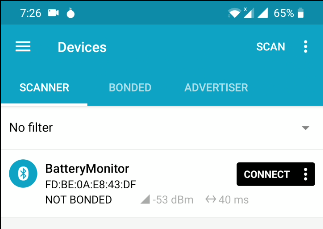
\includegraphics[width=\textwidth]{Bluetooth/BatteryApp}
  \caption{Battery app ``nRF Connect''}    
\end{figure}


Go to that and you will see the services and characteristics of the device.Tap on Battery service and you will the battery levels being read from the Arduino.

%\begin{figure}
%  \includegraphics[width=\textwidth]{Bluetooth/BatteryAppAttention}
%  \caption{Arduino BLE with ``nRF Connect''}    
%\end{figure}


\subsection{Example 2 -- Arduino BLE Accelerometer Tutorial}

I showed you a very easy example to show you jpw you can send simple data via Bluetooth. If you are new to this, try this example first. It will help to give you a better understanding of the BLE.

\subsubsection{Step 1 -- Installing Libraries}

For this example, we will need two libraries 

\begin{itemize}
  \item \FILE{ArduinoBLE} -- To Send Data via Bluetooth
  \item \FILE{LSM9DS1} -- To Read data from inbuilt Accelerometer
\end{itemize}

Both these libraries are available in library manager. Simply search for that using the name and click on install.

\subsubsection{Step 2 -- Test Accelerometer Code (Optional)}

Now we will try running the accelerometer code to make sure that these data are being read properly. For that, use the below code.


\begin{lstlisting}
#include <Arduino_LSM9DS1.h>

void setup() {
    Serial.begin(9600);
    while (!Serial);
    Serial.println("Started");
    
    if (!IMU.begin()) {
        Serial.println("Failed to initialize IMU!");
        while (1);
    }
    
    Serial.print("Accelerometer sample rate = ");
    Serial.print(IMU.accelerationSampleRate());
    Serial.println(" Hz");
    Serial.println();
    Serial.println("Acceleration in G's");
    Serial.println("XtYtZ");
}

void loop() {
    float x, y, z;
    
    if (IMU.accelerationAvailable()) {
        IMU.readAcceleration(x, y, z);
        
        Serial.print(x);
        Serial.print('t');
        Serial.print(y);
        Serial.print('t');
        Serial.println(z);
    }
}
\end{lstlisting}

Once uploaded, start the serial monitor. You will see the data being populated. Try tilting the board in all direction and you will see the value changes accordingly.

\subsubsection{Step 3 -- Upload the Code}

Now its time to upload the complete code. Copy the code below and paste it in the IDE.

\begin{lstlisting}
#include <ArduinoBLE.h>
#include <Arduino_LSM9DS1.h>

int accelX=1;
int accelY=1;
float x, y, z;

BLEService customService("1101");
BLEUnsignedIntCharacteristic customXChar("2101", BLERead | BLENotify);
BLEUnsignedIntCharacteristic customYChar("2102", BLERead | BLENotify);

void setup() {
    IMU.begin();
    Serial.begin(9600); 
    while (!Serial);
    
    pinMode(LED_BUILTIN, OUTPUT);
    
    if (!BLE.begin()) {
        Serial.println("BLE failed to Initiate");
        delay(500);
        while (1);
    }
    
    BLE.setLocalName("Arduino Accelerometer");
    BLE.setAdvertisedService(customService);
    customService.addCharacteristic(customXChar);
    customService.addCharacteristic(customYChar);
    BLE.addService(customService);
    customXChar.writeValue(accelX);
    customYChar.writeValue(accelY);
    
    BLE.advertise();
    
    Serial.println("Bluetooth device is now active, waiting for connections...");
}


void loop() {
    
    BLEDevice central = BLE.central();
    if (central) {
        Serial.print("Connected to central: ");
        Serial.println(central.address());
        digitalWrite(LED_BUILTIN, HIGH);
        while (central.connected()) {
            delay(200);
            read_Accel();
            
            customXChar.writeValue(accelX);
            customYChar.writeValue(accelY);
            
            Serial.print("At Main Function");
            Serial.println("");
            Serial.print(accelX);
            Serial.print(" - ");
            Serial.println(accelY);
            Serial.println("");
            Serial.println("");
        }
    }
    digitalWrite(LED_BUILTIN, LOW);
    Serial.print("Disconnected from central: ");
    Serial.println(central.address());
}

void read_Accel() {
    
    if (IMU.accelerationAvailable()) {
        IMU.readAcceleration(x, y, z);
        accelX = (1+x)*100;
        accelY = (1+y)*100;
        
    }
}
\end{lstlisting}

Select the right port and board. Click on upload.

\subsubsection{Step 4 -- Testing Arduino BLE Accelerometer}

In your Android smartphone, install the app ``nRF Connect''. Open it and start the scanner. You will see the device “Arduino Accelerometer” in the device list. Now tap on connect and a new tab will be opened.

\begin{figure}
    \centering
    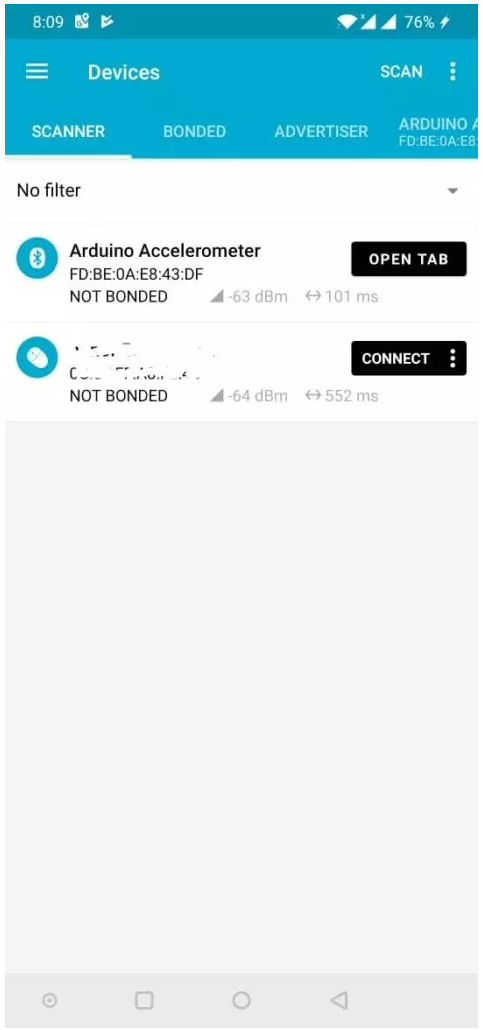
\includegraphics[width=0.6\textwidth]{Bluetooth/BatteryAppAcc}
    \caption{nRF Connect Screen}    
\end{figure}

\begin{figure}
    \centering
    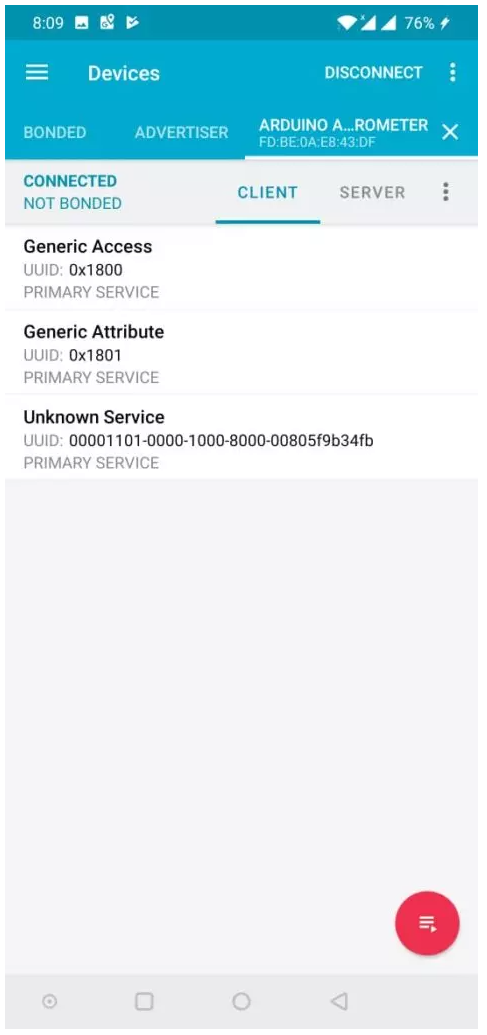
\includegraphics[width=0.6\textwidth]{Bluetooth/BatteryAppAcc2}
    \caption{Accelerometer Values Read from Arduino Using BLE}    
\end{figure}

Go to that and you will see the services and characteristics of the device.

Tap on Unknown Service and you will see the accelerometer values being read from the Arduino.

In the next post, I will show you how you can send inbuilt sensor values such as accelerometer, gyroscope, color sensor and gesture sensor from the Arduino to your phone as well as another Arduino via BLE.









\section{Arduino Library \PYTHON{BLEAK}}

Low Energy (BLE) protocol. BLE allows you to exchange data between devices wirelessly and efficiently. You can use the bleak library in Python to interact with \HREF{https://www.hackster.io/sridhar-rajagopal/control-arduino-nano-ble-with-bluetooth-python-331e33}{BLE devices}.

To get started, you need to install the bleak library using pip:

\medskip

\SHELL{pip install bleak}


\medskip

Then, you need to write a Python program that can scan for BLE devices, connect to the Arduino Nano 33 BLE 33 Sense, and read or write data to its characteristics. Characteristics are the attributes that define the data and behavior of a BLE device. \HREF{https://docs.arduino.cc/tutorials/nano-33-ble-sense/cheat-sheet/}{For example, the Arduino Nano 33 BLE 33 Sense has a characteristic for each color of its RGB LED}.

You can find an example of a Python program that can control the RGB LED of the Arduino Nano 33 BLE 33 Sense using bleak here3. You can also find the corresponding Arduino sketch that sets up the BLE service and characteristics for the Nano 33 BLE 33 Sense here4.


\section{Test}


\section{Test with Bluetooth Module Connection}

The same procedure we need to follow for making the successful bleutooth coonection, the one we follow for on-board sensors. Below figure \ref{fig:testsoftware-fur-bluetooth} shows the ArduinoBLE library in the example section of Arduino IDE.

\begin{center}
    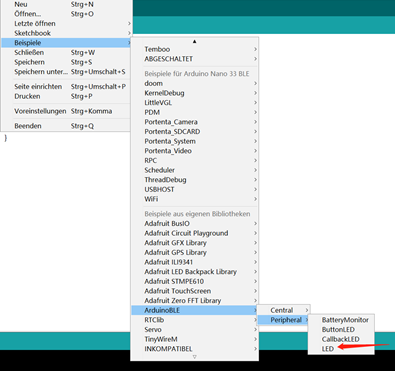
\includegraphics[width=0.7\linewidth]{Nano33BLESense/TestsoftwareBluetooth}
    \captionof{figure}{Bluetooth Connection}
    \label{fig:testsoftware-fur-bluetooth}
\end{center}

Bluetooth wireless technology allows us to share the data, the voice, the music, the video, and a lot of information between paired devices, It is built into many products, from mobile phones, cars to medical devices and computers. It has lower power consumption. It is easily upgradeable. It has range better than Infrared communication. Bluetooth is used for voice and data transfer, we can communicate by recieving and sending the data with other bluetooth connected devices. It is also possible to output a value on the phone side or also on the laptop by making the proper pairing. 





\section{BLEStack}


\begin{center}
    \begin{tikzpicture}
        % First Rectangle
        \draw[black, fill=LightBlue!50, rounded corners] (1,0) rectangle (12,2);
        \node[black, align=center] at (6.5,1) {%
            Application \\
            Profiles and Services
        };
        
        % 2nd Rectangle
        \draw[black!90, fill=LightBlue, rounded corners] (0,-1.5) rectangle (14,-15.5);
        
        
        
        % First Inner Rectangle
        \draw[black!90, fill=LightBlue, rounded corners] (0.5,-2.5) rectangle (13.5,-10);
        \node[black, align=center] at (13,-3) {%
            Host
        };
        
        % First Row
        % First Inner Rectangle
        \draw[black!90, fill=LightBlue!50, rounded corners] (2.5,-3) rectangle (5.5,-5);
        \node[black, align=center] at (4,-4) {%
            Generic Attribute \\
            Profile (GATT)
        };
        
        % Second Inner Rectangle
        \draw[black!90, fill=LightBlue!50, rounded corners] (6,-3) rectangle (12,-5);
        \draw[black!90, fill=LightBlue!50, rounded corners] (9.5,-3) rectangle (12,-9.5);
        \draw[LightBlue!50, fill=LightBlue!50 ] (9.4,-3.01) rectangle (9.6,-4.99);
        \node[black, align=center] at (9,-4) {%
            Generic Access Profile \\
            (GAP)
        };
        
        % Second Row
        % Third Inner Rectangle
        \draw[black!90, fill=LightBlue!50, rounded corners] (2.5,-5.5) rectangle (5.5,-7.5);
        \node[black, align=center] at (4,-6.5) {%
            Attribute Protocol \\
            (ATT)
        };
        
        % Fourth Inner Rectangle
        \draw[black!90, fill=LightBlue!50, rounded corners] (6,-5.5) rectangle (9,-7.5);
        \node[black, align=center] at (7.5,-6.5) {%
            Security Manager \\
            (SM)
        };
        
        % Third Row
        % Fifth Inner Rectangle
        \draw[black!90, fill=LightBlue!50, rounded corners] (1,-8) rectangle (9,-9.5);
        \node[black, align=center] at (5,-8.75) {%
            Logical Link COntrol and Application Layer \\
            Protocol (L2CAP)
        };
        
        
        
        % Second Inner Rectangle
        \draw[black!90, fill=LightBlue, rounded corners] (0.5,-10.5) rectangle (13.5,-15);
        \node[black, align=center] at (12.5,-11) {%
            Controller
        };
        
        %2.0 First Inner Rectangle
        \draw[black!90, fill=LightBlue!50, rounded corners] (0.8,-11) rectangle (11.5,-12.5);
        \node[black, align=center] at (6,-11.75) {%
            Link Layer (LL)
        };
        %2.0 First Inner Rectangle
        \draw[black!90, fill=LightBlue!50, rounded corners] (0.8,-13) rectangle (11.5,-14.5);
        \node[black, align=center] at (6,-13.75) {%
            Physical Layer (PHY)
        };
        
        % Add arrow
        % \draw [<->, >=Stealth, black!10] (1.75,0) -- (1.75,-8);
        \draw [line width=4pt, black!20, <->, >=Stealth, fill=black!10] (1.75,0) -- (1.75,-8);
        \draw [line width=4pt, black!20, <->, >=Stealth, fill=black!10] (4,0) -- (4,-3);
        \draw [line width=4pt, black!20, <->, >=Stealth, fill=black!10] (9,0) -- (9,-3);
        
        
    \end{tikzpicture}
    
\end{center}

